\documentclass{article}
\usepackage[utf8]{inputenc}

\documentclass[a4paper]{article}
\usepackage[12pt]{extsizes}
\usepackage{amsmath,amsthm,amssymb}
\usepackage[hidelinks]{hyperref} 
\usepackage[warn]{mathtext}
\usepackage[T1,T2A]{fontenc}
\usepackage[utf8]{inputenc}
\usepackage[english,russian]{babel}
\usepackage{tocloft}
\linespread{1.5}
\usepackage{indentfirst}
\usepackage{setspace}
%\полуторный интервал
\onehalfspacing

\newcommand{\RomanNumeralCaps}[1]
    {\MakeUppercase{\romannumeral #1}}

\usepackage{amssymb}

\usepackage{graphicx, float}
\graphicspath{{pictures/}}
\DeclareGraphicsExtensions{.pdf,.png,.jpg}
\usepackage[left=25mm,right=1cm,
    top=2cm,bottom=20mm,bindingoffset=0cm]{geometry}
\renewcommand{\cftsecleader}{\cftdotfill{\cftdotsep}}

\addto\captionsrussian{\renewcommand{\contentsname}{СОДЕРЖАНИЕ}}
\addto\captionsrussian{\renewcommand{\listfigurename}{СПИСОК ИЛЛЮСТРАЦИЙ}}

\usepackage{fancyhdr}
\usepackage[nottoc]{tocbibind}

\fancypagestyle{plain}{
\fancyhf{}
\renewcommand{\headrulewidth}{0pt}
\fancyhead[R]{\thepage}
}

\usepackage{blindtext}
\pagestyle{myheadings}
\usepackage{hyperref}

\begin{document}
\begin{titlepage}
  \begin{center}
    \large
    Санкт-Петербургский политехнический университет Петра Великого
    
    Институт прикладной математики и механики
    
    \textbf{Высшая школа прикладной математики и вычислительной физики}
    \vfill
    \textsc{\textbf{\Large{Отчёт по лабораторной работе №8}}}\\[5mm]
    \\ по дисциплине
    \\ <<Математическая статистика>>\\
\end{center}

\vfill

\begin{tabular}{l p{140} l}
Выполнила студентка \\группы 3630102/80401 && Мамаева Анастасия Сергеевна \\
\\
Проверил\\Доцент, к.ф.-м.н.& \hspace{0pt} &   Баженов Александр Николаевич \\\\
\end{tabular}

\hfill \break
\hfill \break
\begin{center} Санкт-Петербург \\2021 \end{center}
\thispagestyle{empty}
\end{titlepage}
\newpage
\newpage
\begin{center}
    \setcounter{page}{2}
    \tableofcontents
\end{center}
\newpage
\begin{center}
    \setcounter{page}{3}
    \listoffigures
\end{center}

\newpage

\section {Постановка задачи}
\noindent Провести дисперсионный анализ с применением крритерия Фишера по данным регистраторов для одного сигнала. Определить области однородности сигнала, переходные области, шум/ фон. Длину сигнала взять равной 1024.

\section{Теория}
\noindent Необходимо вычислить следующие величины:
\begin{enumerate}
    \item Внутригрупповая дисперсия 
    \begin{equation}
        s_{IntaGroup}^{2} = \frac{1}{k} \sum_{i=1}^{k} s_i^{2} = \frac{1}{k} \sum_{i=1}^{k} \frac{\sum_{j=1}^{n} (x_{ij}-X_{ср})^{2}}{k-1}
    \end{equation}
где $X_{ср}$ -- среднее для части выборки; $k$ -- количество частей выборки; $n$ -- количество элементов в рассматриваемой части выборки. Внутригрупповая дисперсия является дисперсией совокупности и рассматривается как среднее значение выборочных дисперсий.
\item Межгрупповая дисперсия
\begin{equation}
        s_{InterGroup}^{2}  = k \frac{\sum_{i=1}^{k} (X_{i_{ср}}-X_{ср})^{2}}{k-1}
    \end{equation}
где $X_{1_{ср}}, X_{2_{ср}}, \dots, X_{k_{ср}}$ -- среднее значение для под-выборок, $X_{ср}$ -- среднее значение этих мредних значений под-выборок.
\item Значение критерия Фишера
\begin{equation}
    F=\frac{s_{InterGroup}^{2}}{s_{IntaGroup}^{2}}
\end{equation}
\end{enumerate}

\section{Ход работы}
\noindent На начальном этапе необходимо извлечь сигнал из исходных данных
(wave-ampl.txt). Известно, что сигнал имеет длину 1024, поэтому необходимо
выбрать начальный индекс, кратный 1024.\\\\
\noindent Далее необходимо построить гистограмму, столбцы отвечают за
следующие подобласти:
\begin{itemize}
    \item фон (столбец с наименьшим значением)
    \item переходы (столбцы с малыми значениями)
    \item сигнал (второй по величине столбец после фона)
\end{itemize}
\noindent Перед определением областей однородности, необходимо устранить
явные выбросы. Для этого был использован медианный фильтр (выброс =
среднее арифметическое его соседей). По итогу получим сглаженный сигнал.
После устранения выбросов необходимо разделить сигнал на области
(сигнал, фон, переходные процессы). \\\\
\noindent Как только области получены, необходимо определить их тип. Это
осуществляется с помощью применения критерия Фишера. Если значение
критерия Фишера велико, это будут переходные процессы, если же значение
находится вблизи 1, то эти области однородны.

\section{Программная реализация}
\noindent Лабораторная работа выполнена на языке Python вресии 3.7 в среде разработки JupyterLab. Использовались дополнительные библиотеки:
 \begin{enumerate}
        \item matplotlib (визуализация)
        \item numpy (вычисление ряда числовых характеристик)
    \end{enumerate}
В приложении находится ссылка на GitHub репозиторий с исходныи кодом.

\section{Результаты}
\noindent В работе рассматривался сигнал с индексом 1.
	\begin{figure}[H]
		\centering
		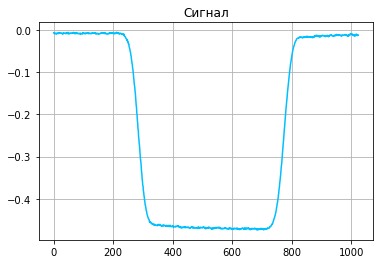
\includegraphics[width = 13cm, height = 8cm]{Signal.png}
		\caption{Изображение входного сигнала}
		\label{fig:sP}
	\end{figure}
	
		\begin{figure}[H]
		\centering
		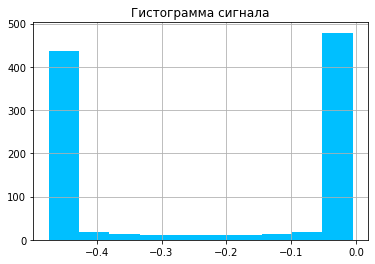
\includegraphics[width = 13cm, height = 8cm]{hist.png}
		\caption{Гистограмма сигнала}
		\label{fig:sP}
	\end{figure}
	
	\begin{figure}[H]
		\centering
		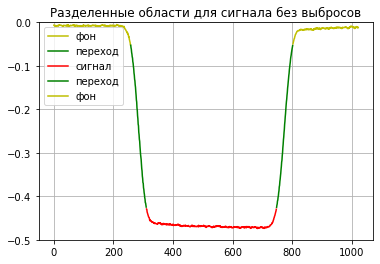
\includegraphics[width = 13cm, height = 8cm]{Areas.png}
		\caption{Разделение областей для данных сигнала с устранением выбросов}
		\label{fig:sP}
	\end{figure}

\begin{table}[H]
    \centering
    \begin{tabular}{|c|c|c|c|}
    \hline
        Промежуток & Тип & Кол-во разбиений & критерий Фишера  \\ \hline
        1 & фон & 6 & 0.68\\ \hline
        2 & переход & 6 & 45.42 \\ \hline
        3 & сигнал & 19 & 0.04\\ \hline
        4 & переход & 5 & 32.38\\ \hline
        5 & фон & 4 & 0.97\\ \hline
    \end{tabular}
    \caption{Характеристики выделенных областей}
    \label{tab:my_label}
\end{table}

\section{Обсуждение}
\begin{enumerate}
    \item Для входных данных сигнала были получены следующие области
однородности: фон (слева и справа) и сигнал, эти области
однородны так как значения критерия Фишера находится вблизи 1
\item На переходах значения критерия Фишера много больше 1,
следовательно, эти области неоднородны
\end{enumerate}

\section{Приложение}
\noindent Код программы GitHub URL:\\
\newline https://github.com/Brightest-Sunshine/Math-Statistic-2021/blob/main/Lab8/Lab8.ipynb

\begin{thebibliography}{9}
\bibitem{book1} Гланц, С. Медико-Биологическая статистика. Пер. с англ. — М.,
Практика, 1998
\bibitem{book2} Электронный ресурс. Виды дисперсий.
https://math.semestr.ru/group/types-variances.php
\end{thebibliography}

\end{document}

